% ==============================================================================
% CAPÍTULO 05 - PROPUESTA DE PROYECTO
% ==============================================================================

\chapter{Propuesta de Proyecto}
\label{cap:propuesta_proyecto}
\justifying

\section{Descripción General de la Propuesta}

La propuesta consiste en el desarrollo de una plataforma web integral orientada a la gestión digital de quejas y denuncias para la DDP del IPN. El sistema tiene como finalidad modernizar y optimizar los procesos institucionales relacionados con el registro, validación, seguimiento, análisis y resolución de expedientes, mediante el uso de tecnologías de automatización, centralización documental y análisis inteligente de información.

La plataforma busca sustituir diversos procesos manuales y fragmentados que actualmente dificultan la operación eficiente de la DDP, permitiendo establecer un entorno digital centralizado para la administración de expedientes, evidencias y comunicaciones institucionales.

Asimismo, la solución incorpora componentes tecnológicos orientados al fortalecimiento de la trazabilidad, seguridad y transparencia del proceso de atención, integrando mecanismos de control de acceso, seguimiento de actividades y administración estructurada de información sensible.

De igual manera, el sistema contempla la integración de un componente inteligente basado en técnicas de Procesamiento de Lenguaje Natural y aprendizaje automático, cuya finalidad es asistir en la clasificación preliminar de las quejas conforme a criterios institucionales previamente establecidos.

\section{Objetivo de la Plataforma}

La plataforma tiene como objetivo proporcionar una solución tecnológica integral que permita optimizar los procesos internos de gestión de quejas y denuncias dentro de la DDP, mejorando la eficiencia operativa, reduciendo tiempos administrativos y fortaleciendo la organización institucional de la información.

Asimismo, el sistema busca centralizar el ciclo de vida completo de los expedientes digitales, desde el registro inicial de la queja hasta la conclusión formal del procedimiento, garantizando trazabilidad, disponibilidad y resguardo seguro de la información.

Adicionalmente, la solución pretende apoyar al personal administrativo y jurídico mediante herramientas de automatización y análisis inteligente que faciliten la clasificación preliminar de los casos, la validación de información y la gestión documental.

\section{Componentes Principales del Sistema}

La propuesta contempla distintos módulos funcionales orientados a cubrir las necesidades operativas y administrativas de la DDP.

\subsection{Portal del Quejoso}

Permite a los usuarios registrar nuevas quejas, adjuntar evidencias digitales, consultar el estado de sus expedientes, descargar acuses y mantener seguimiento de sus trámites mediante una interfaz accesible y centralizada.

\subsection{Módulo Administrativo}

Integra las herramientas necesarias para la gestión interna de expedientes por parte de las diferentes áreas institucionales, incluyendo recepción, primer contacto, subDDP, DDP y administración técnica.

\subsection{Clasificador Inteligente}

Incorpora un sistema de clasificación automática basado en técnicas de Procesamiento de Lenguaje Natural y aprendizaje automático, orientado a apoyar la determinación preliminar de competencia institucional a partir de la narrativa textual proporcionada por el usuario.

\subsection{Expediente Digital}

Centraliza toda la información relacionada con cada expediente, incluyendo documentos, evidencias, actuaciones, acuerdos, notificaciones y resoluciones, permitiendo mantener trazabilidad completa del procedimiento.

\subsection{Sistema de Seguridad y Control de Acceso}

Implementa mecanismos de autenticación, autorización basada en roles, auditoría de actividades y protección de información sensible, garantizando seguridad y confidencialidad durante la operación del sistema.

\section{Arquitectura General de la Solución}

La solución propuesta se encuentra basada en una arquitectura híbrida de microservicios, diseñada para proporcionar modularidad, escalabilidad y mantenibilidad a los distintos componentes del sistema.

La arquitectura contempla la separación de responsabilidades mediante servicios independientes especializados, permitiendo desacoplar los procesos administrativos, la gestión documental, el manejo de usuarios y el componente inteligente de clasificación automática.

Asimismo, la plataforma incorpora un API Gateway encargado de centralizar la comunicación entre los diferentes microservicios, facilitando el control de seguridad, monitoreo y administración de solicitudes.

El backend principal del sistema se desarrolla utilizando Java y Spring Boot, mientras que el componente de clasificación inteligente se implementa mediante herramientas de Python orientadas al procesamiento de lenguaje natural y aprendizaje automático.

Por otra parte, la persistencia de información se realiza mediante PostgreSQL, incorporando mecanismos de manejo de datos estructurados y semi-estructurados para garantizar flexibilidad y eficiencia en la administración de expedientes digitales.

\begin{figure}[H]
    \centering
    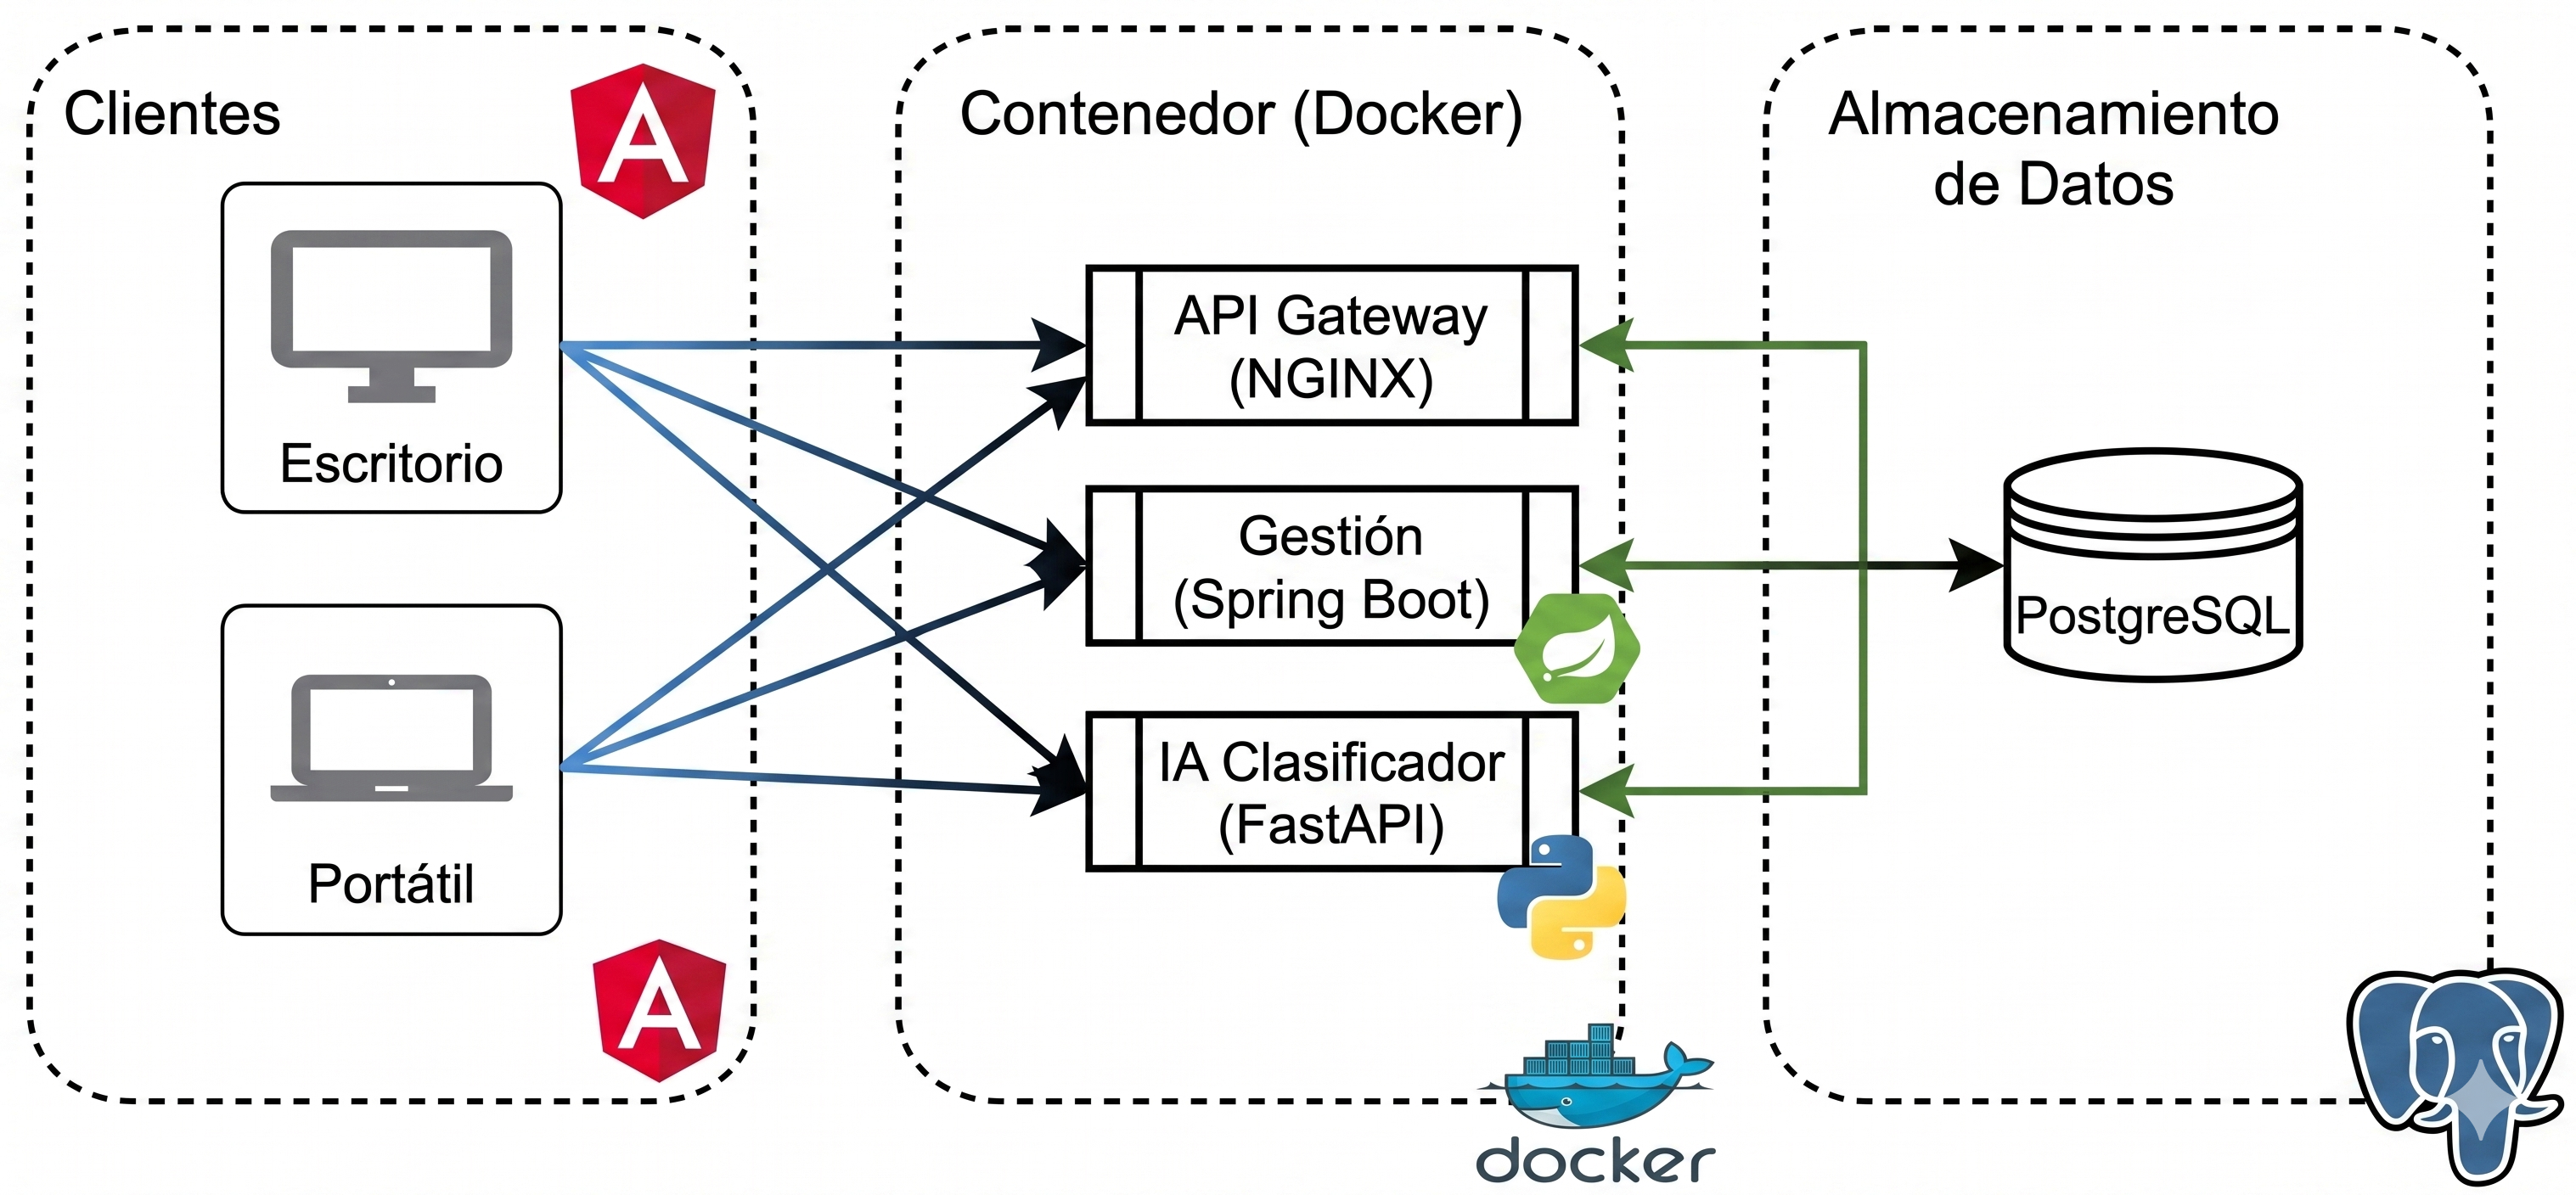
\includegraphics[width=0.95\textwidth]{imagenes/documento/diagrama_microservicios.png}
    \caption{Arquitectura general propuesta para la plataforma institucional.}
    \label{fig:arquitectura_general}
\end{figure}

\section{Funcionalidades Principales}

La plataforma integra diversas funcionalidades orientadas a fortalecer la operación institucional y mejorar la experiencia de los usuarios.

\begin{itemize}

    \item Registro digital de quejas y denuncias.

    \item Gestión de evidencias digitales y documentación asociada.

    \item Seguimiento del estado de expedientes en tiempo real.

    \item Generación automática de folios y acuses de recibo.

    \item Administración centralizada de expedientes digitales.

    \item Clasificación preliminar automática de quejas mediante inteligencia artificial.

    \item Control de acceso basado en roles institucionales.

    \item Gestión de notificaciones y comunicaciones internas.

    \item Generación de reportes y estadísticas institucionales.

    \item Auditoría y trazabilidad de actividades dentro del sistema.

\end{itemize}

\section{Innovación Tecnológica}

Uno de los principales elementos innovadores de la propuesta corresponde a la integración de técnicas de Procesamiento de Lenguaje Natural y aprendizaje automático dentro de un entorno institucional de gestión de quejas y denuncias.

La incorporación de un clasificador inteligente permite analizar automáticamente las narrativas textuales proporcionadas por los usuarios, apoyando la identificación preliminar de competencia institucional y facilitando la canalización de expedientes.

Asimismo, la solución integra una arquitectura híbrida distribuida basada en microservicios, permitiendo separar componentes operativos, administrativos e inteligentes dentro de un entorno escalable y modular.

De igual manera, la propuesta incorpora mecanismos modernos de seguridad, trazabilidad y control documental orientados al manejo seguro de información sensible y evidencias digitales.

La centralización del expediente digital, junto con la automatización de procesos operativos y administrativos, contribuye a fortalecer la eficiencia institucional y mejorar la capacidad de respuesta de la DDP.

\section{Beneficios Esperados}

La implementación de la plataforma permitirá generar beneficios tanto operativos como tecnológicos e institucionales.

Entre los principales beneficios esperados se encuentran:

\begin{itemize}

    \item Reducción de tiempos administrativos en la atención de quejas.

    \item Disminución del rezago operativo mediante automatización de procesos.

    \item Mejora en la trazabilidad y seguimiento de expedientes.

    \item Centralización segura de información y evidencias digitales.

    \item Optimización de la comunicación entre áreas institucionales.

    \item Apoyo inteligente para la clasificación preliminar de casos.

    \item Incremento en la transparencia y control de actividades.

    \item Fortalecimiento de la seguridad y privacidad de la información.

    \item Generación de estadísticas e indicadores institucionales.

    \item Mejora en la experiencia digital de los usuarios.

\end{itemize}

\section{Alcance de la Propuesta}

La propuesta contempla el desarrollo de una plataforma web integral capaz de administrar el registro, seguimiento y gestión de expedientes digitales relacionados con quejas y denuncias presentadas ante la DDP.

El sistema incluye funcionalidades orientadas al manejo de usuarios, control de accesos, administración documental, seguimiento de expedientes, notificaciones y clasificación preliminar automatizada de las quejas.

Asimismo, la solución contempla la integración de herramientas de apoyo inteligente para asistir al personal administrativo y jurídico durante las etapas iniciales del análisis de competencia institucional.

Sin embargo, el sistema no busca sustituir la toma de decisiones jurídicas ni reemplazar la intervención del personal especializado de la DDP. Las resoluciones, dictámenes y determinaciones finales continúan siendo responsabilidad de las autoridades institucionales correspondientes.

Finalmente, el alcance de la propuesta se limita al fortalecimiento tecnológico y operativo de los procesos internos relacionados con la gestión de quejas y denuncias dentro del entorno institucional de la DDP.

\section{Costo del proyecto}
Debemos tener en cuenta que el desarrollo de la presente plataforma requiere una inversión planificada. A fin de garantizar la viabilidad económica del proyecto, se realizó un análisis detallado de los recursos necesarios, considerando los gastos operativos reales de cada integrante del equipo, las herramientas especializadas requeridas por el stack tecnológico seleccionado y el capital humano involucrado durante un horizonte de doce meses. La siguiente tabla presenta el resumen consolidado de dicha inversión, organizada por categoría de gasto.
\begin{table}[h!]
\centering
\caption{Resumen consolidado de la inversión (12 meses)}
\begin{tabular}{|l|r|c|}
\hline
\textbf{Categoría} & \textbf{Costo Total (MXN)} & \textbf{Porcentaje (\%)} \\ \hline
Hardware (Inversión Inicial)            & \$34{,}999.00    & 3.48\%  \\ \hline
Servicios Individuales (Luz e Internet) & \$24{,}708.00    & 2.46\%  \\ \hline
Licenciamiento y VPS                    & \$52{,}761.60    & 5.25\%  \\ \hline
Capital Humano y Capacitación           & \$892{,}657.50   & 88.81\% \\ \hline
\textbf{COSTO TOTAL DEL PROYECTO}       & \textbf{\$1{,}005{,}126.10} & \textbf{100.00\%} \\ \hline
\end{tabular}
\end{table}

Como podemos observar el 88.81\% de la inversión se concentra en Capital Humano.